%
%
\documentclass[10pt,a4paper,oneside]{book}

%Hello there. Don't know what to do?
	%Search for the %? or \fixme and fix/add stuff.
	%Check zapiski 2007, your notes and your memory and fix/add stuff
	%kul knjige imajo quote na začetku poglavij
%
%lol, windows newline bug poje to vrsto včasih :P
%\documentclass[10pt,a4paper,oneside]{book}

\usepackage[slovene]{babel}
\usepackage[utf8x]{inputenc}
\usepackage[fleqn]{amsmath}%fleqn - levo zamaknjene enačbe
\usepackage{amsfonts}
\usepackage{amssymb}
\usepackage{makeidx}
\usepackage{graphicx}
\usepackage[x11names, rgb]{xcolor}
\usepackage{tikz}
\usetikzlibrary{calc,automata,snakes,arrows,shapes,decorations.text,positioning,shapes.arrows,chains}

\usepackage{torstyle}
%?this feels too much like CSS hacks :(
%torstlye predloge:
%Definicija \Def{}
%Primer \Primer{}
%Prirejen itemize \begin{items}
\hypersetup{pdftitle={Teoretične osnove računalništva}}

\begin{document}
\begin{titlepage}
\begin{center}
%looks useful
%{\resizebox{15cm}{!}{Teoretične osnove računalništva}}\\[5pt]
\ \\[1cm]
{\Huge\bf Teoretične osnove računalništva}\\[1cm]
{\huge \today}\ \\[1.5cm]
%{\LARGE Zapiski predavanj 2010/2011}\\[15pt]%Odkar sem dodal kontekstno-odvisne in linearne, to ni več to :P
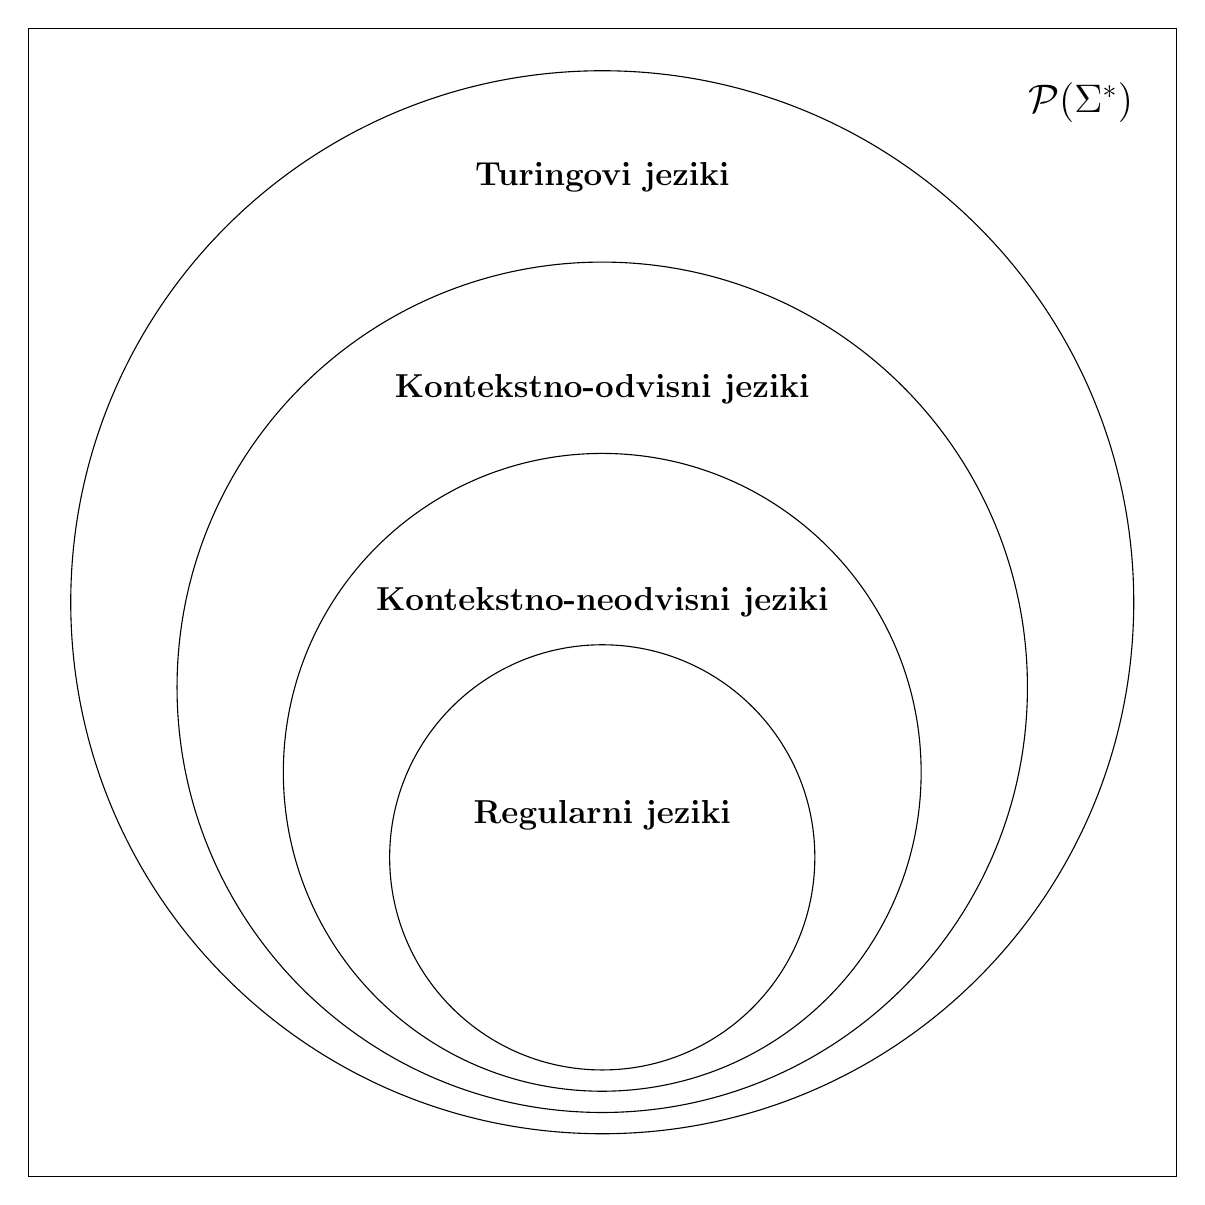
\begin{tikzpicture}[scale=1.35]
	\draw (-5.4cm,-5.4cm) rectangle (5.4cm,5.4cm);
	\node at (4.5cm,4.7cm) {\Large $\mathcal{P}(\Sigma^*)$};%sva šla vprašat... ker \Sigma^* znajo že RJ opisat, samo ne vseh možnih ;)

	\draw (0cm,0cm) circle (5cm);
	\node at (0,4cm) {\large\bf {Turingovi jeziki}};

	\draw (0cm,-0.8cm) circle (4cm);
	\node at (0,2cm) {\large\bf {Kontekstno-odvisni jeziki}};

	\draw (0cm,-1.6cm) circle (3cm);
	\node at (0,0cm) {\large\bf {Kontekstno-neodvisni jeziki}};

	\draw (0cm,-2.4cm) circle (2cm);
	\node at (0,-2cm) {\large\bf {Regularni jeziki}};
\end{tikzpicture}

\vfill
\parbox{7.5cm}{
\begin{center}

\includegraphics[width=0.15\textwidth]{./CC}\\[6pt]

This work is licensed under a Creative Commons Attribution-NonCommercial-ShareAlike 3.0 Unported License
\end{center}
}

\end{center}
\end{titlepage}
\tableofcontents
\pagebreak
%\newpage

\chap{Vaja 1 (4. 3. 2011)}
\sect{Turingovi stroji - zapisi definicijo, delta funkcijo, in opis trenutnega stanja}

Turingov stroj sestavljajo:
\begin{items}
\item Nadzorno enoto (glava)
\item Čitalno okno (roka in vid)
\item Trak (papir)
\end{items}
V postopku formalizacije, pa je zaradi večje preprostosti, zahteval še, da je stroj sestavljen iz končno mnogo elementov, ter da deluje v diskretnih korakih.%?končno mnogo elementov? na kaj to cilja? zidar: mislm da koncno stanj, koncno trakov, dimezij, itd ..
\ \\
\begin{center}
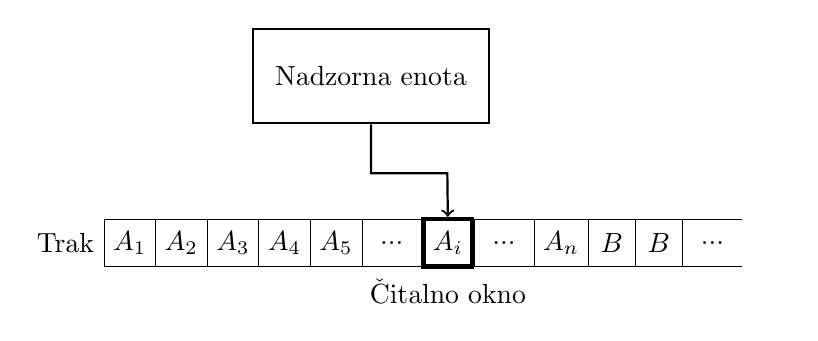
\begin{tikzpicture}[start chain, node distance=-0.075mm, thick, cell/.style={draw, very thin, on chain, minimum size=0.6cm}]
	\node (Trak) [on chain] {Trak};
	\foreach \x in {1,2,...,5} {
		\node ({A\x}) [cell] {$A_{\x}$};
	}
	\node ({Ad1}) [cell] {\ ...\ \ };
	\node ({Ai}) [cell, ultra thick] {$A_i$};
	\node ({Ad2}) [cell] {\ ...\ \ };
	\node ({An}) [cell] {$A_n$};
	\node ({Ab1}) [cell] {$B$};
	\node ({Ab2}) [cell] {$B$};
	\node ({Ad3}) [cell] {\ ...\ \ };
	\node ({end}) [cell, draw=white] {};

	%?must be a better way, zadnja črta niti ni naravnost
	\node (ne) at (110bp, 60bp) [draw, minimum height=1.2cm, minimum width=3cm]  {Nadzorna enota};
	\draw (ne.south) -- (110bp, 25bp) -- (137.5bp, 25bp) [->] to (Ai.north);
	\node [below] at (Ai.south) {Čitalno okno};
\end{tikzpicture}
\end{center}

\Def{Turingov stroj je definiran kot sedmerka $M=\langle Q, \Sigma, \Gamma, \delta, q_0, B, F \rangle $, kjer je:
\begin{items}
	\item $Q$ končna množica stanj
	\item $\Sigma$ končna množica vhodnih simbolov, $Q \cap \Sigma = \emptyset$
	\item $\Gamma$ končna množica tračnih simbolov, $\Sigma \subset \Gamma$
	\item $\delta$ funkcija prehodov: $Q \times \Gamma \rightarrow Q \times \Gamma \times \{L,D\}$,\\ kjer $L$ in $D$ označujeta premik levo ali desno
	\item $q_0$ začetno stanje, $q_0 \in Q$
	\item $B$ prazen simbol, $B \in \Gamma$
	\item $F$ množica končnih stanj, $F \subseteq Q$ 
\end{items}}
Stroj deluje tako, da v vsakem koraku opravi naslednje:
\begin{items}
	\item preide v neko stanje
	\item zapiše nov simbol v celico, ki je pod oknom
	\item okno premakne eno celico levo ali desno
\end{items}

\Def{Trenutni opis $TO = \Gamma^* \times Q \times \Gamma^*$ je množica vseh trenutnih opisov.\\
Nek trenutni opis $\langle \alpha_1, q, \alpha_2 \rangle$, ali krajše $\alpha_1\ q\ \alpha_2$ opisuje konfiguracijo Turingovega stroja.}
\fixme naredi bolj formalen zapis, z besedo na traku in stanjem. (k je tist iz isrm neki govoru



\sect{Naredi turingov stroj za $L = \lbrace 0,00,000 \rbrace $}

Opis risanja turingovis strojev ki uporabljamo na vajah.
Napišemo stanja avtomata (ko rešujemo probamo čim manj optimizirati - združevati stanja - ker tako najhitreje naredimo napako), in po puščicah se premikamo v druga stanja, in na pučšici napišemo spremembo stanja v obliki $ X \rightarrow Y,\lbrace D, L \rbrace$. $X$ je znak prebran v oknu, $Y$ znak ki ga zapisemo v okno, $D$ ali $L$ prestavlja smer premika okna. \\[1.2em]

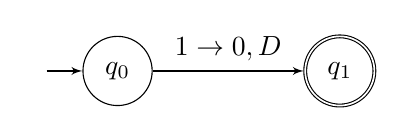
\begin{tikzpicture}[>=latex',/tikz/initial text=""]
	\node (q0) at (0bp,0bp)  [state, initial]   {$q_0$};
	\node (q1) at (80bp,0bp) [state, accepting] {$q_1$};

	\draw [left,->] (q0) to node[auto] {$ 1 \rightarrow 0, D $} (q1);
\end{tikzpicture}
\\[1.2em]
In zdej lahko probamo narisati ta TS:
\\[1.2em]
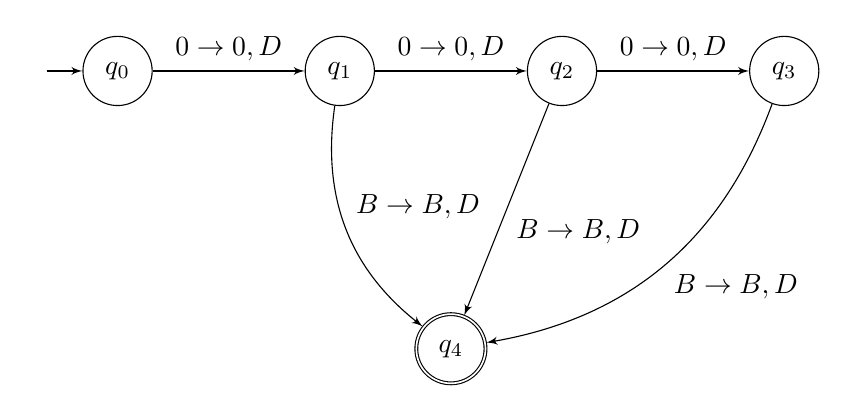
\begin{tikzpicture}[>=latex',/tikz/initial text=""]
	\node (q0) at (0bp,0bp)  [state, initial]   {$q_0$};
	\node (q1) at (80bp,0bp) [state] {$q_1$};
	\node (q2) at (160bp,0bp) [state] {$q_2$};
	\node (q3) at (240bp,0bp) [state] {$q_3$};
	\node (q4) at (120bp,-100bp) [state, accepting] {$q_4$};

	\draw [left,->] (q0) to node[auto] {$ 0 \rightarrow 0, D $} (q1);
	\draw [left,->] (q1) to node[auto] {$ 0 \rightarrow 0, D $} (q2);
	\draw [left,->] (q2) to node[auto] {$ 0 \rightarrow 0, D $} (q3);

	\draw [bend right,->] (q1) to node[auto] {$ B \rightarrow B, D $} (q4);
	\draw [left,->] (q2) to node[auto] {$ B \rightarrow B, D $} (q4);
	\draw [bend left,->] (q3) to node[auto] {$ B \rightarrow B, D $} (q4);


\end{tikzpicture}

\sect{Naredi turingov stroj za $L = \lbrace 0^n10^n \ | \ n > 0 \rbrace  $}
Delovanje si zamislimo tako nekako:
\begin{items}
	\item premikamo se od leve do desne, in pisemo $B$ namesto 0
	\item zadevo ponavljamo dokler ne pridemo do $1$
	\item če preberemo $1$, preverimo če sta na levi in desni strani $b$ 
	\item nato se premaknemo v končno stanje
\end{items}
\ \\[1.2em]
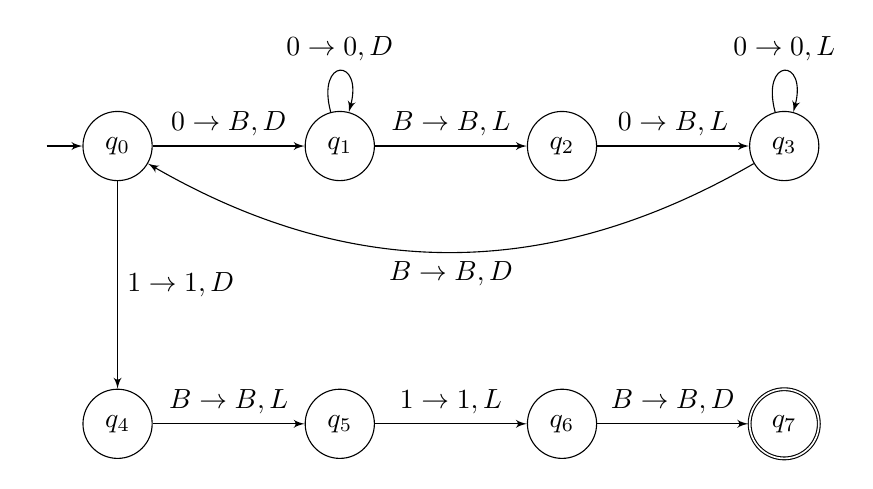
\begin{tikzpicture}[>=latex',/tikz/initial text=""]
	\node (q0) at (0bp,0bp)  [state, initial]   {$q_0$};
	\node (q1) at (80bp,0bp) [state] {$q_1$};
	\node (q2) at (160bp,0bp) [state] {$q_2$};
	\node (q3) at (240bp,0bp) [state] {$q_3$};
	\node (q4) at (0bp,-100bp) [state] {$q_4$};
	\node (q5) at (80bp,-100bp) [state] {$q_5$};
	\node (q6) at (160bp,-100bp) [state] {$q_6$};
	\node (q7) at (240bp,-100bp) [state, accepting] {$q_7$};

	\draw [left,->] (q0) to node[auto] {$ 0 \rightarrow B, D $} (q1);
	\draw [loop above,->] (q1) to node[auto] {
		$0 \rightarrow 0, D $
		% kako naredim dve vrstici tuki? manjka	$1 \rightarrow 1, D $
		} (q1);
	\draw [left,->] (q1) to node[auto] {$ B \rightarrow B, L $} (q2);
	\draw [left,->] (q2) to node[auto] {$ 0 \rightarrow B, L $} (q3);
	\draw [loop above,->] (q3) to node[auto] {$ 0 \rightarrow 0, L $
		% isto ? manjka	$1 \rightarrow 1, L $
		} (q3);
	\draw [bend left,->] (q3) to node[auto] {$ B \rightarrow B, D $} (q0);

	\draw [left,->] (q0) to node[auto] {$ 1 \rightarrow 1, D $} (q4);
	\draw [left,->] (q4) to node[auto] {$ B \rightarrow B, L $} (q5);
	\draw [left,->] (q5) to node[auto] {$ 1 \rightarrow 1, L $} (q6);
	\draw [left,->] (q6) to node[auto] {$ B \rightarrow B, D $} (q7);


\end{tikzpicture}


\sect{Naredi turingov stroj za $L = \lbrace ww^R \ | \ w \in \lbrace 0,1 \rbrace^* \rbrace $}

\sect{Naredi turingov stroj za $L = \lbrace ww  \ | \ w \in \lbrace 0,1 \rbrace^* \rbrace $}



\chap{Vaja 2 (7. 3. 2011)}
\sect{Turingovi stroji - nadaljevanje}



\end{document}